%% -*- coding: utf-8 -*-
\documentclass[12pt,a4paper]{scrartcl} 
\usepackage[utf8]{inputenc}
\usepackage[english,russian]{babel}
\usepackage{indentfirst}
\usepackage{misccorr}
\usepackage{graphicx}
\usepackage{amsmath}
\begin{document}
\section{Введение}
\label{sec:intro}

% Что должно быть во введении
\begin{enumerate}
 \item Обработка данных в системе 1С:Университет
 \item Этапы заполнения данных
 \item Скриншоты программы
\end{enumerate}
\section{Ход работы}
\label{sec:exp}

\subsection{Этапы заполнения данных}

\label{sec:exp:code}
\begin{verbatim}
При заполнении ведомостей необходимо:
1. Выбрать нужный факультет, форму обучение, курс(1-4).(1).
2. В открывшемся окне будет отображен список ведомостей.
   Выбрав нужную аттестационную ведомость, по предмету и форме оценивания.
   Заходим в неё.(2)
   Пример представлен на рис.1
\end{verbatim}
\begin{verbatim}
В открывшемся окне аттестационной ведомости необходимо:
1. Изменить дату проведения экзамана (зачета).(1). 
2. Ещё раз извеняем дату, там же в в параметрах 
   Единица измерения - надо выбрать часы (с кодом 0000000001).(2).
3. Во вкладке, список обучающихся необходимо проверить:
-  Всех студентов по списку на бумажном носителе.
   Если кого-то не хватает, нажимаем кнопку "добавить" или клавишей "insert".(3).   
   После этого действия появиться пустая строчка, чтоб добавить человека,
   двойным щелчком нажимаем по пустой строке, в конце строки можно увидеть "...".
   Нажав на три точки, откроеться окно со списком всех студентов,
   это окно можно окгрыть горячей клавищей "F4". Далее выбираем нужного студента
   двойным щелчком кнопки мыши добавляем студента, затем он будет отображен в списке.
   Примечание ~ Если сразу в пустой строке вносить ФИО студента,
   он (она) будут отображены, но некоректно, т.к не будет номера зачеткой книжки.
4. Далее выбираем систему оценивания пятибальную или двубальную.(4).   
5. Затем когда все студенты добавленны или удалены из ведомости,
   в окне "Отметка" сверяясь с бумажным носителем вбиваем оценки,
   зачет, незачет, неявка, удовлетворительно, хорошо, отлично.(5).
   Когда все данные по студентам внесены, переходим в вкладку преподователи.
   Сверяя с бумажным носителем, добавляем преподователя как описано в (3) пункте.
   Далее необходимо проверить правельность внесенных данных,
   если все верно, жмем кнопку "Провести и закрыть".
   Пример представлен на рис.2
\end{verbatim}

\subsection {Скриншоты программы}
\begin{figure}[h]
	\centering
	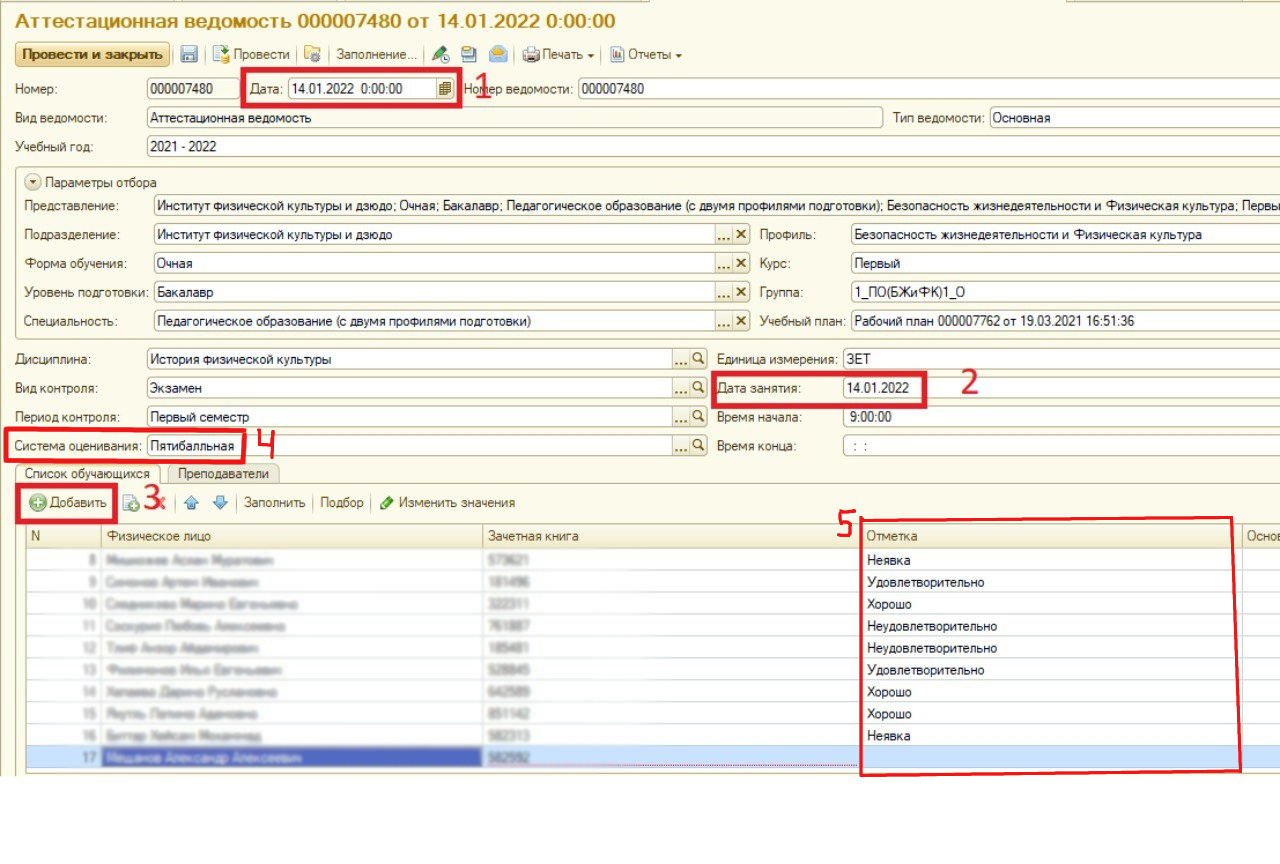
\includegraphics[width=1 \textwidth]{Vedom 2}
	\caption{Главная стр.}\label{fig:par}
\end{figure}
\begin{figure}[h]
	\centering
	\includegraphics[width=1 \textwidth]{ведомость 2,1.jpg}
	\caption{Внутренние данные ведомости}\label{fig:par}
\end{figure}
\end{document}
